\chapter{Clustering Algorithm and Application}
\label{chapter:clustering}

The objective of classification is to find assignments between data points and categories. For some applications this can be done by taking correctly labelled data and comparing a new data point to the data points in different categories to see which category best fits. One such algorithm is k-nearest-neighbour. In our context the issue with this approach is that the data is only labelled as to which experiment it came from, e.g. positive control in human cells, negative control in mouse cells. However, as noted before not all cells from these experiments behaved as we expected them to, e.g. some cells activated in the negative control or did not activate in the positive control. Therefore, we choose to use a clustering algorithm which does not have the need for classified training data.

\section{Gaussian Mixture Model}
\label{sec:gaussian_mixture_model}

This section follows the article Gaussian Mixture Model by Reynolds~\cite{reynolds2009}.

Often gathered observations are distributed as a normal distribution. These distributions have a density function
\begin{align*}
	g(x|\mu, \Sigma) = \frac{1}{(2\pi)^{D/2} |\Sigma|^{1/2}} exp\left( - \frac{1}{2} (x-\mu)^T \Sigma^{-1} (x-\mu) \right)
\end{align*}
with parameters $D$ called the dimension, $\mu$ called the mean vector and $\Sigma$ called the covariance matrix.

As we are concerned with clustering data points we expect the observed data points from different clusters to have different parameters in the normal distribution they come from. Assuming we have $n$ different data sources gives us normal distributions $g_i(x|\mu_i, \Sigma_i)$ where $i=1, ..., n$. Additionally, we might have more data points being generated from some normal distributions while less from others. We can express this using another weight parameter $w_i$ with $i=1, ..., n$. To normalize the weights we set the constraint $\sum w_i = 1$.

The distribution describing the entire dataset now can be described with the distribution
\begin{align}
	\label{eq:sum_of_normal}
	p(x) = \sum_{i=1}^{n} w_i g(x|\mu_i, \Sigma_i).
\end{align}

Gaussian Mixture Model is a method to retrieve these parameters $w_i$, $\mu_i$ and $\Sigma_i$ for some $D$ dimensional data points generated from $n$ normal distributions.

From these parameters it is easy to cluster the data as we know where data points from the different clusters are expected to lie.

From equation~\ref{eq:sum_of_normal} we expect every $\Sigma_i$ to be independent of each other. In the context of Gaussian Mixture Models this is called having a full covariance matrix. However, we can eliminate some of the variables in the covariance matrix if we choose a diagonal covariance matrix. Additionally, we might specify to use the same covariance matrix for all $i$, which is called tied in this context.

Choosing a full covariance matrix is not necessary even if the data is expected to have statistically independent features, as the overall density is compromised from multiple normal distributions with diagonal $\Sigma_i$. This enables us to model correlations between features.

The question now is how we can derive the parameters $w_i, \mu_i$ and $\Sigma_i$. We choose the approach which chooses the parameters where the likelihood that the data was generated by these parameters is maximal. This is known as maximum likelihood estimation. The likelihood can be expressed as

\begin{align*}
	L(w_i, \mu_i, \Sigma_i|X) = p(X|w_i, \mu_i, \Sigma_i) = \prod_{t=1}^n p(x_t|w_i, \mu_i, \Sigma_i)
\end{align*}

with $X = (x_1, ..., x_n)$ being the recorded data. As $L(w_i, \mu_i, \Sigma_i|X)$ is non-linear in the parameters deriving the maximum is not trivial. Instead, we use an iterative approach which approaches the solution. Define $\lambda = (w_i, \mu_i, \Sigma_i)$. Simplifying to a diagonal covariance matrix gives us the iterative algorithm where we define the successor values $\bar{.}$ as

\begin{align*}
	Pr(i | x_t, \lambda) := \frac{w_i g(x_t | \mu_i, \Sigma_i)}{\sum_{k=1}^{n} w_k g(x_t | \mu_k, \Sigma_k)}\\
	\bar{w}_i := \frac{1}{n} \sum_{t=1}^{n} Pr(i | x_t, \lambda)\\
	\bar{\mu}_i := \frac{\sum_{t=1}^{n} Pr(i | x_t, \lambda) x_t}{\sum_{t=1}^{n} Pr(i | x_t, \lambda)}\\
	\bar{\sigma}_i^2 := \frac{\sum_{t=1}^{n} Pr(i | x_t, \lambda) x_t^2}{\sum_{t=1}^{n} Pr(i | x_t, \lambda)} - \bar{\mu}_i^2.
\end{align*}

for $w_i$, $\mu_i$ and $\sigma_i^2$ respectively. One can show that with this iteration rule we have $p(X|\bar{\lambda}) \geq p(X|\lambda)$. The value $Pr(i|x_t, \lambda)$ is known as the a posteriori probability for the i-th component.

% https://scikit-learn.org/stable/modules/mixture.html#gmm

\section{Implementation of the Clustering Algorithm}

Python offers an implementation of Gaussian Mixture Model with the sklearn package. The function with parameters relevant to us is \texttt{sklearn.mixture.GaussianMixture(n\_components, covariance\_type)}. The number of components \texttt{n\_components} can be any positive integer. The \texttt{covariance\_type} can be one of \texttt{‘full’, ‘tied’, ‘diag’} or \texttt{‘spherical’} and describes what type of covariance matrix is used.

As the input of the Gaussian Mixture Model we use data points of the form \texttt{[a, u, d, k1, k2, w1, w2]}, where \texttt{a, u, ..., w2} are the parameters of the approximation from chapter~\ref{chapter:approximating}. As our goal is to separate data points from the four data sets mouse cells and human cells each with a negative and a positive control, we use all particles as input. The pseudo code below describes the steps performed to reach a clustering of the data.

\begin{algorithm}[H] \label{alg:separate}
	\SetAlgoLined
	\DontPrintSemicolon
	\LinesNumbered
	\SetKwInOut{Input}{input}
	\SetKwInOut{Output}{output}
	\caption{Separate}
	
	\Input{parameters of the approximations of all particles in all data sets}
	\Output{assignments to different clusters for each particle, means and standard deviation of each cluster}
	
	\BlankLine
	\Begin{
		initialize Gaussian Mixture by specifying \texttt{n\_components} and \texttt{covariance\_type}\;
		apply Gaussian Mixture to matrix of all parameters of the approximations of all particle data sets\;
		assign particles to clusters according to Gaussian Mixture results\;
		compare asignments from Gaussian Mixture to those of the data set the data stems from\;
		\Return{assignments to clusters, means and standard deviations of every cluster}
	}
\end{algorithm}
\vspace{1cm}

When comparing different covariance types in the Gaussian Mixture we see that using \texttt{‘diag’} we have the lowest error rate. The details are shown in table~\ref{tab:covariance_type_comparison}. Why reducing the number of parameters in the covariance matrix can yield better results is described in section~\ref{sec:gaussian_mixture_model}.

\begin{table}[h!]
	\centering
	\begin{tabular}{|c|c|}
		\hline
		\texttt{full}: $13.23\%$ & \texttt{tied}: $12.7\%$ \\
		\hline
		\texttt{diag}: $7.17\%$ & \texttt{spherical}: $31.52\%$ \\
		\hline
	\end{tabular}
	\label{tab:covariance_type_comparison}
	\caption{Error as a percentage of particles being assigned the wrong component.}
\end{table}

Using a diagonal covariance matrix we can now try to separate the four data sets and visualize the results. As the data is 7 dimensional we show lower dimensional representations of the data both as it is assigned according to the data set it stems from as well as the assignment from algorithm~\ref{alg:separate}. The results can be seen in figure~\ref{fig:vis_output_seperate}.

\begin{figure}
	\centering
	\begin{subfigure}{0.49\textwidth}
		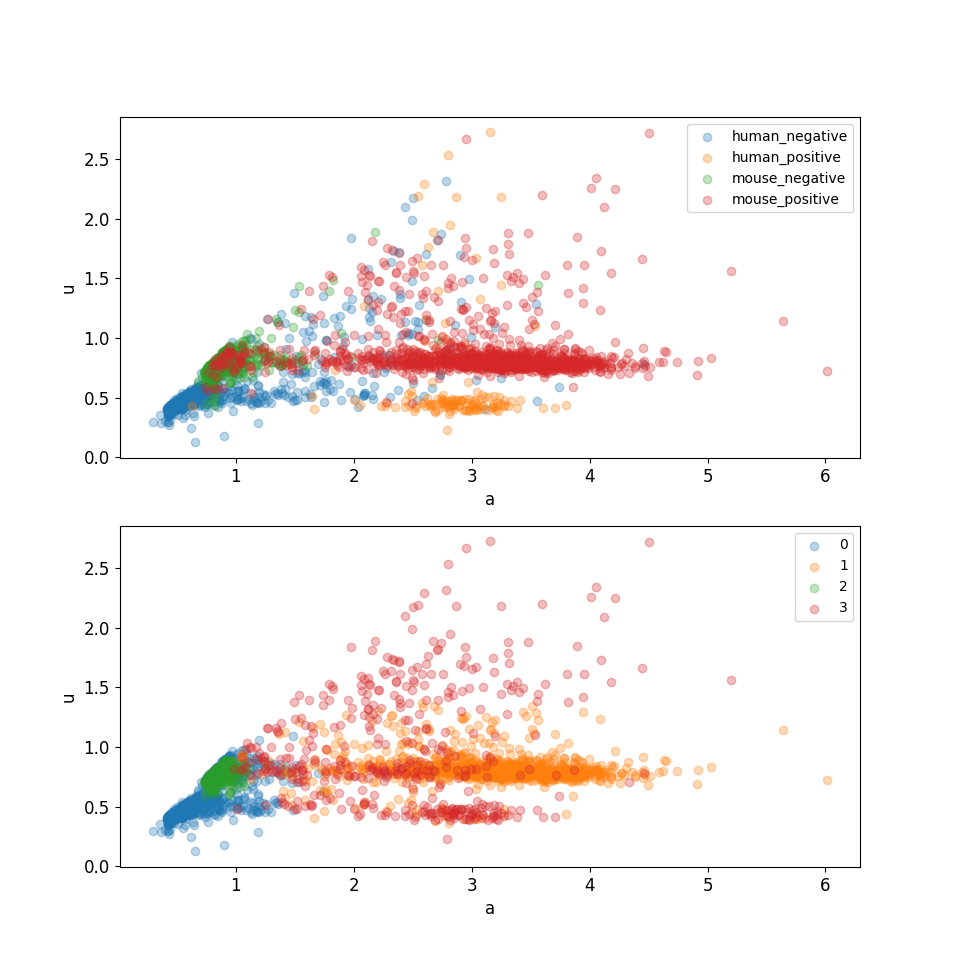
\includegraphics[width=\textwidth]{fig/seperate_a_u}
	\end{subfigure}
	\hfill
	\begin{subfigure}{0.49\textwidth}
		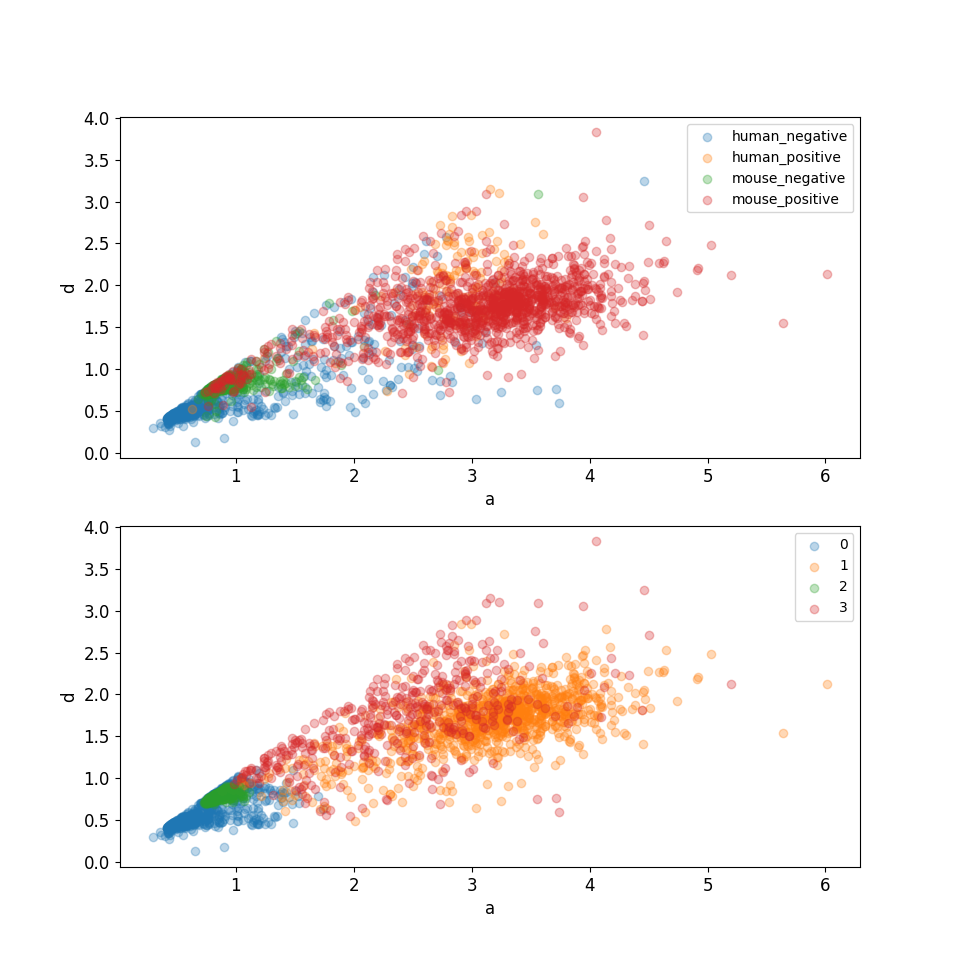
\includegraphics[width=\textwidth]{fig/seperate_a_d}
	\end{subfigure}
	\hfill
	\begin{subfigure}{0.49\textwidth}
		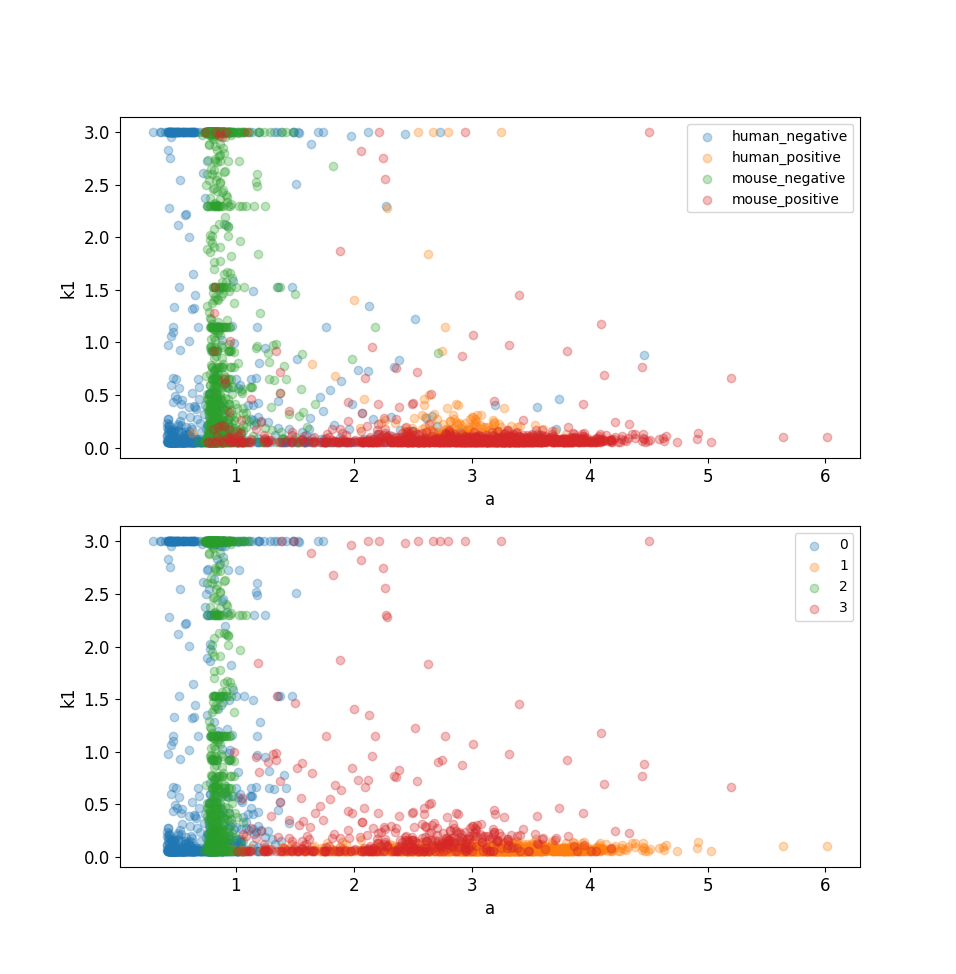
\includegraphics[width=\textwidth]{fig/seperate_a_k1}
	\end{subfigure}
	\hfill
	\begin{subfigure}{0.49\textwidth}
		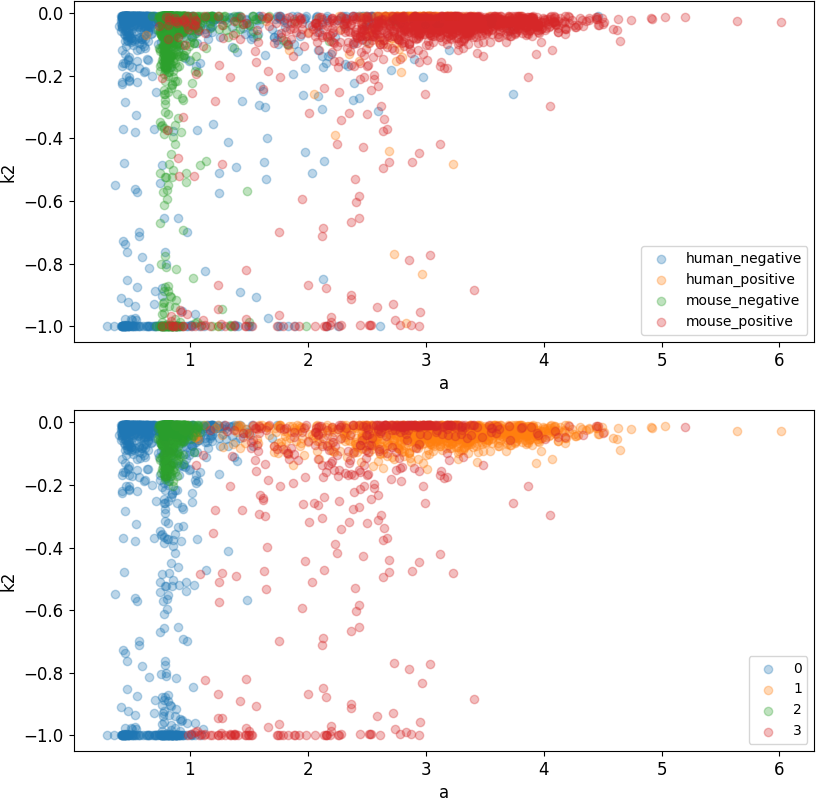
\includegraphics[width=\textwidth]{fig/seperate_a_k2}
	\end{subfigure}
	
	\caption{Visualization of the clustered data points. Each pair of images depicts the clustering according to positive and negative control on either humans of mouse t cells in the upper image and the clustering according to the algorithm proposed in the lower image.}
\label{fig:vis_output_seperate1}
\end{figure}
	
\begin{figure}
	\begin{subfigure}{0.49\textwidth}
		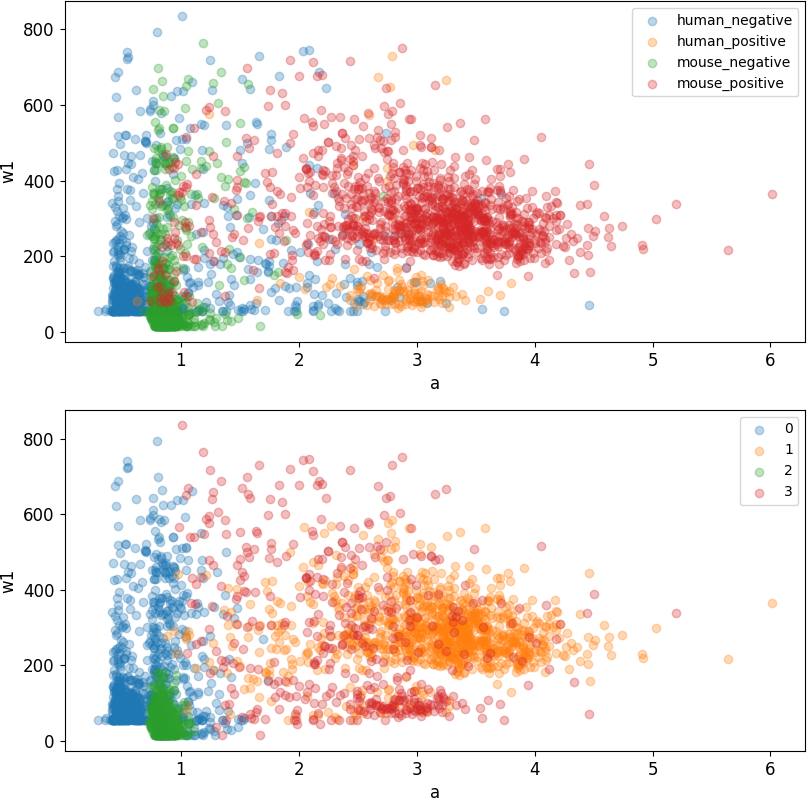
\includegraphics[width=\textwidth]{fig/seperate_a_w1}
	\end{subfigure}
	\hfill
	\begin{subfigure}{0.49\textwidth}
		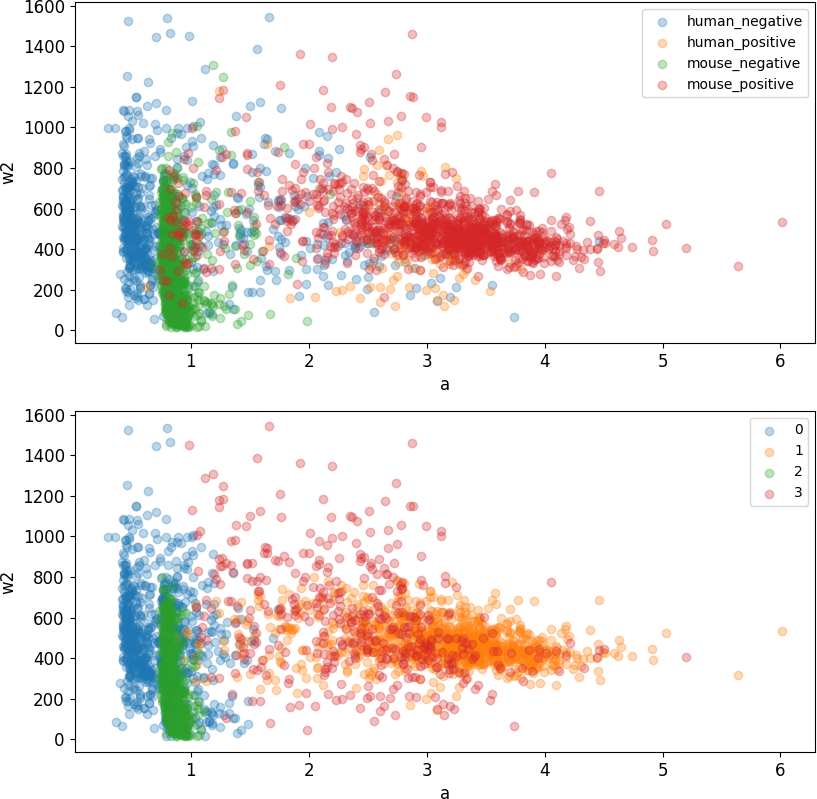
\includegraphics[width=\textwidth]{fig/seperate_a_w2}
	\end{subfigure}
	\hfill
	\begin{subfigure}{0.49\textwidth}
		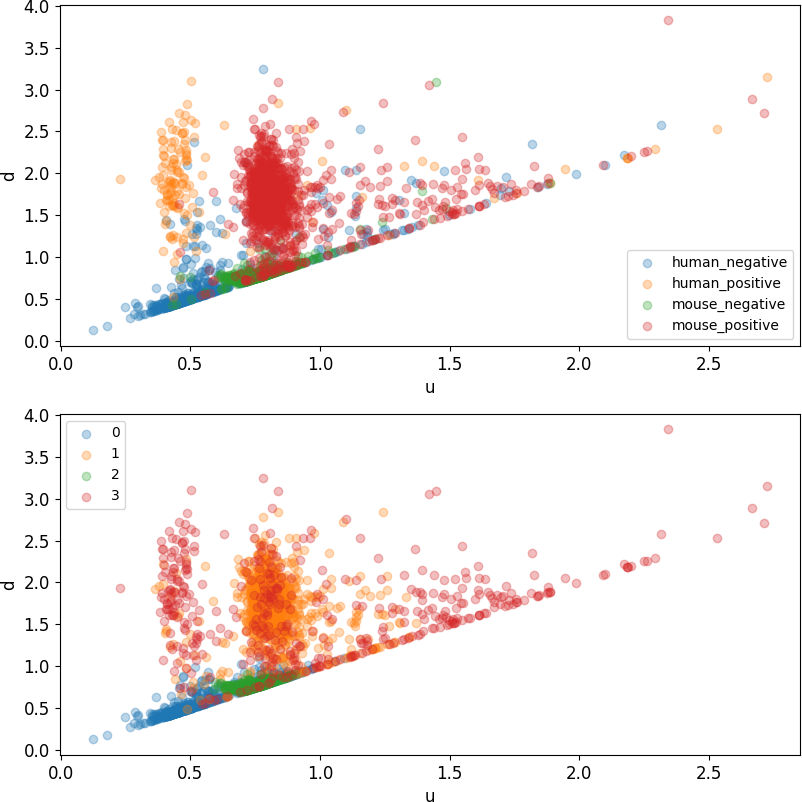
\includegraphics[width=\textwidth]{fig/seperate_u_d}
	\end{subfigure}
	\hfill
	\begin{subfigure}{0.49\textwidth}
		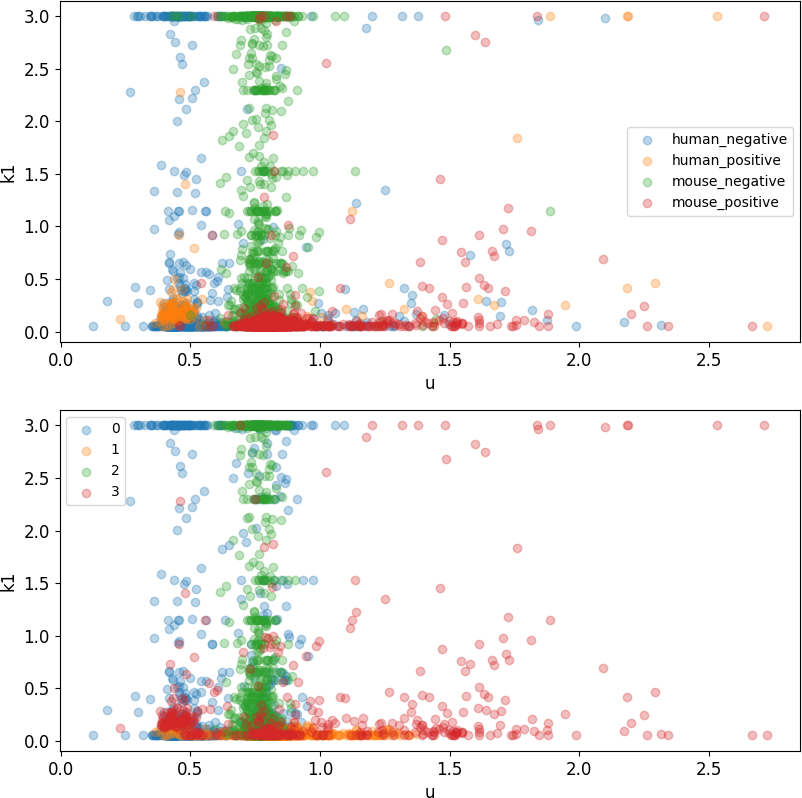
\includegraphics[width=\textwidth]{fig/seperate_u_k1}
	\end{subfigure}
	\hfill
	\begin{subfigure}{0.49\textwidth}
		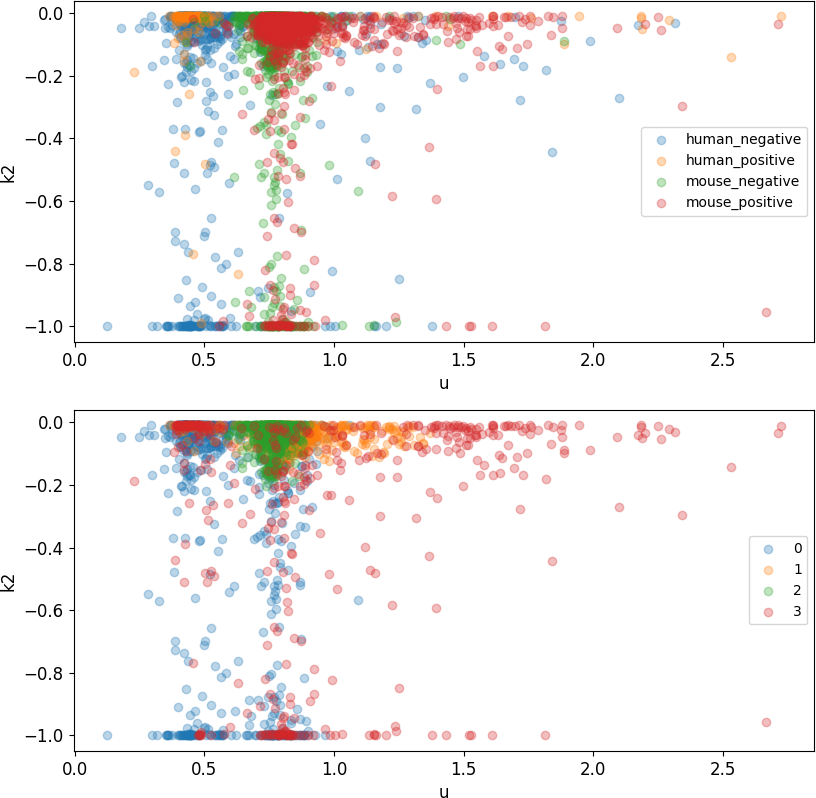
\includegraphics[width=\textwidth]{fig/seperate_u_k2}
	\end{subfigure}
	\hfill
	\begin{subfigure}{0.49\textwidth}
		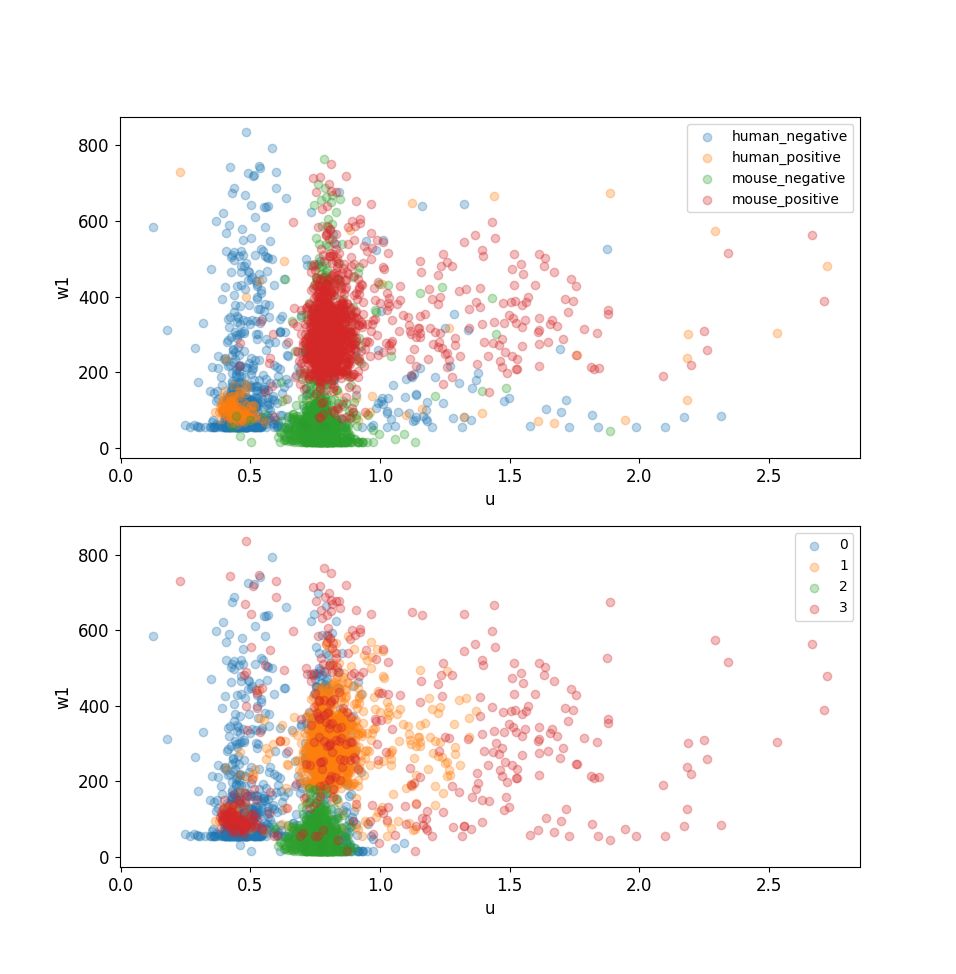
\includegraphics[width=\textwidth]{fig/seperate_u_w1}
	\end{subfigure}
	\caption{Continuation of the visualization of the clustering results.}
\label{fig:vis_output_seperate2}
\end{figure}

\begin{figure}
	\begin{subfigure}{0.49\textwidth}
		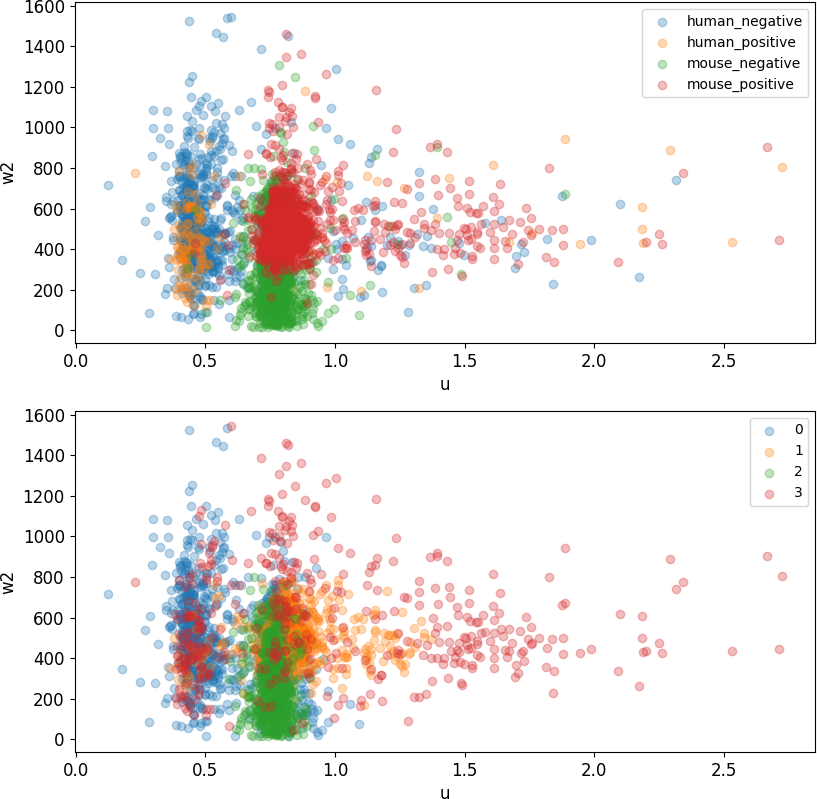
\includegraphics[width=\textwidth]{fig/seperate_u_w2}
	\end{subfigure}
	\hfill
	\begin{subfigure}{0.49\textwidth}
		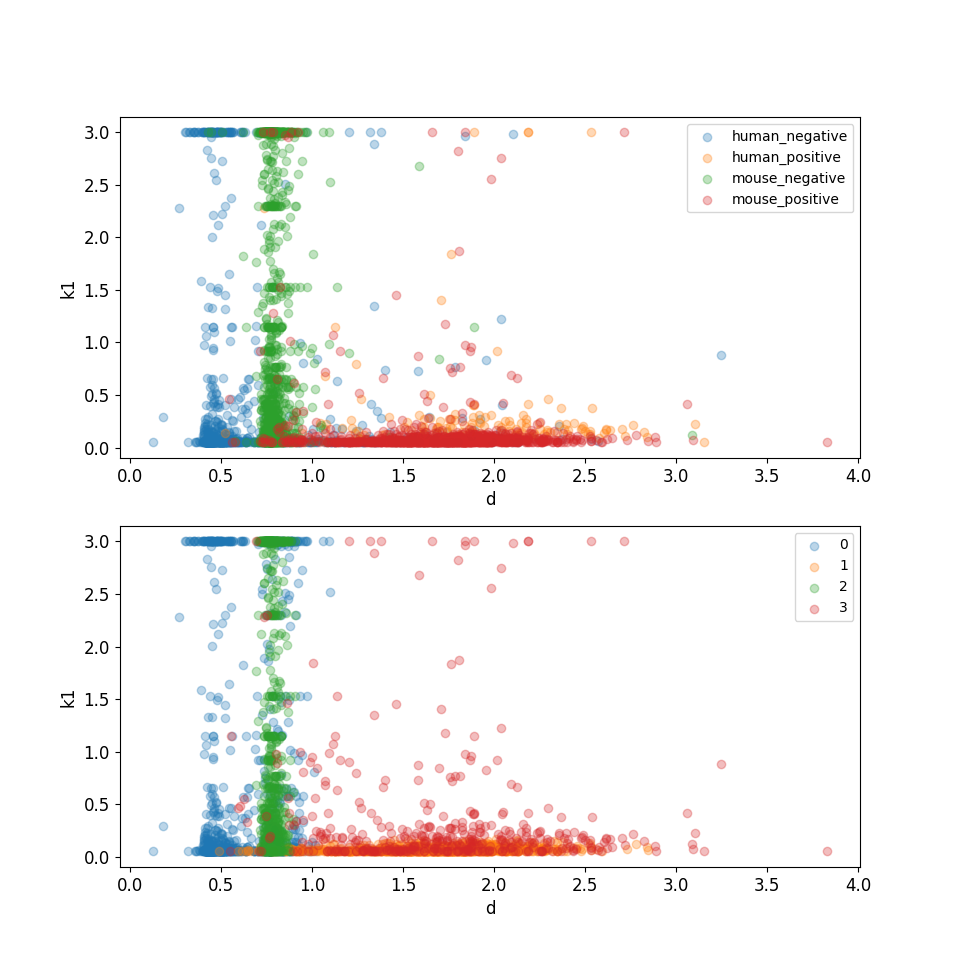
\includegraphics[width=\textwidth]{fig/seperate_d_k1}
	\end{subfigure}
	\hfill
	\begin{subfigure}{0.49\textwidth}
		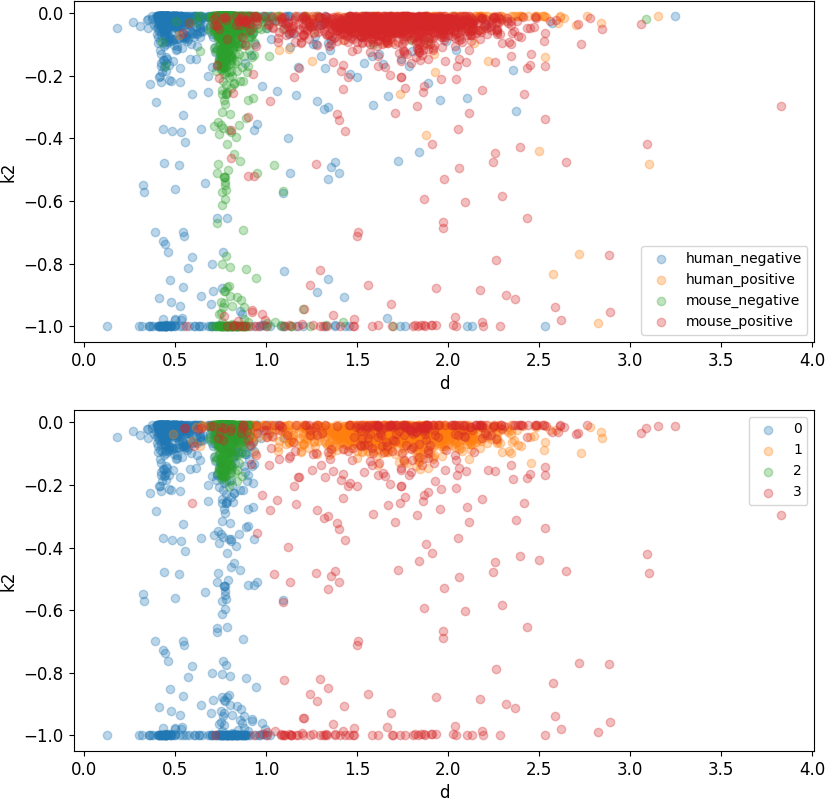
\includegraphics[width=\textwidth]{fig/seperate_d_k2}
	\end{subfigure}
	\hfill
	\begin{subfigure}{0.49\textwidth}
		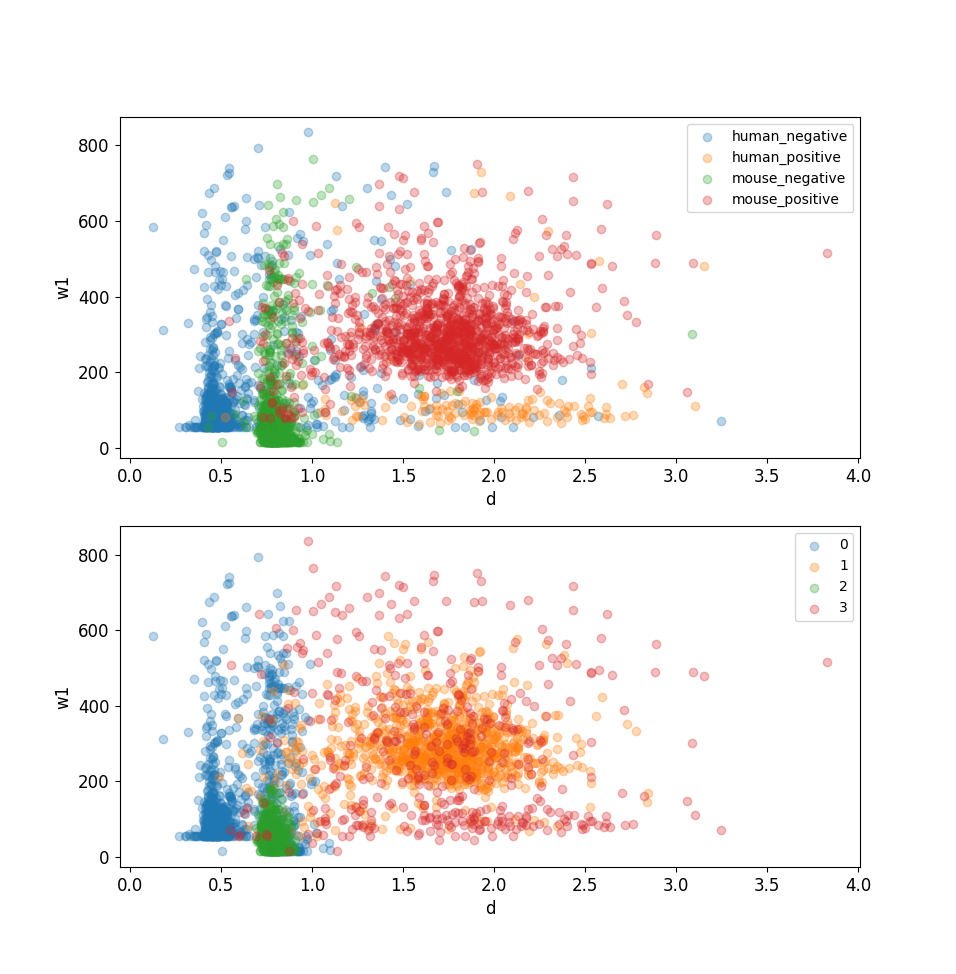
\includegraphics[width=\textwidth]{fig/seperate_d_w1}
	\end{subfigure}
	\hfill
	\begin{subfigure}{0.49\textwidth}
		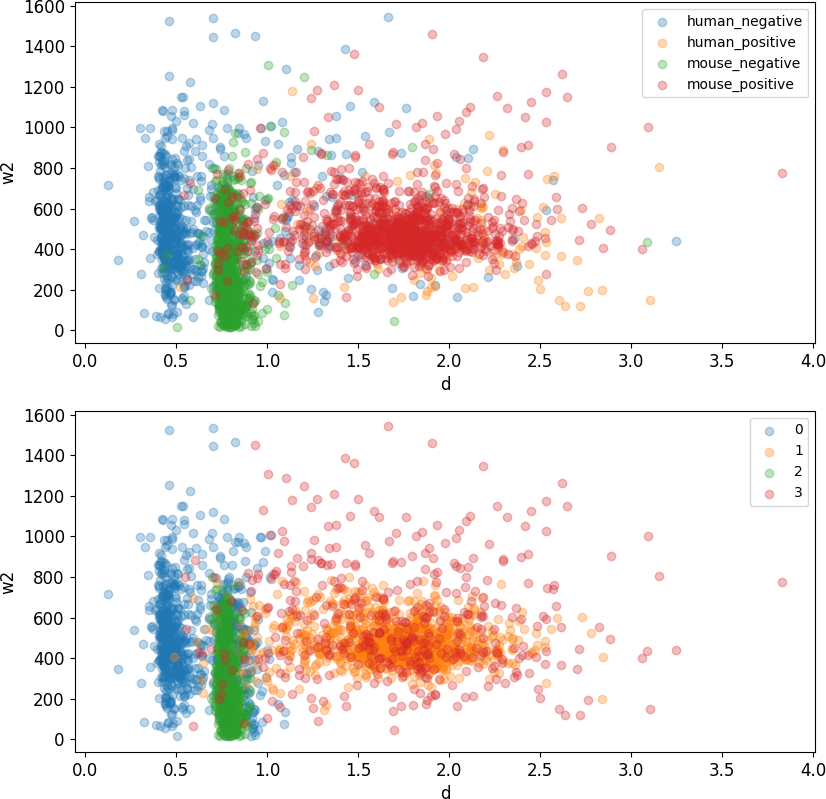
\includegraphics[width=\textwidth]{fig/seperate_d_w2}
	\end{subfigure}
	\hfill
	\begin{subfigure}{0.49\textwidth}
		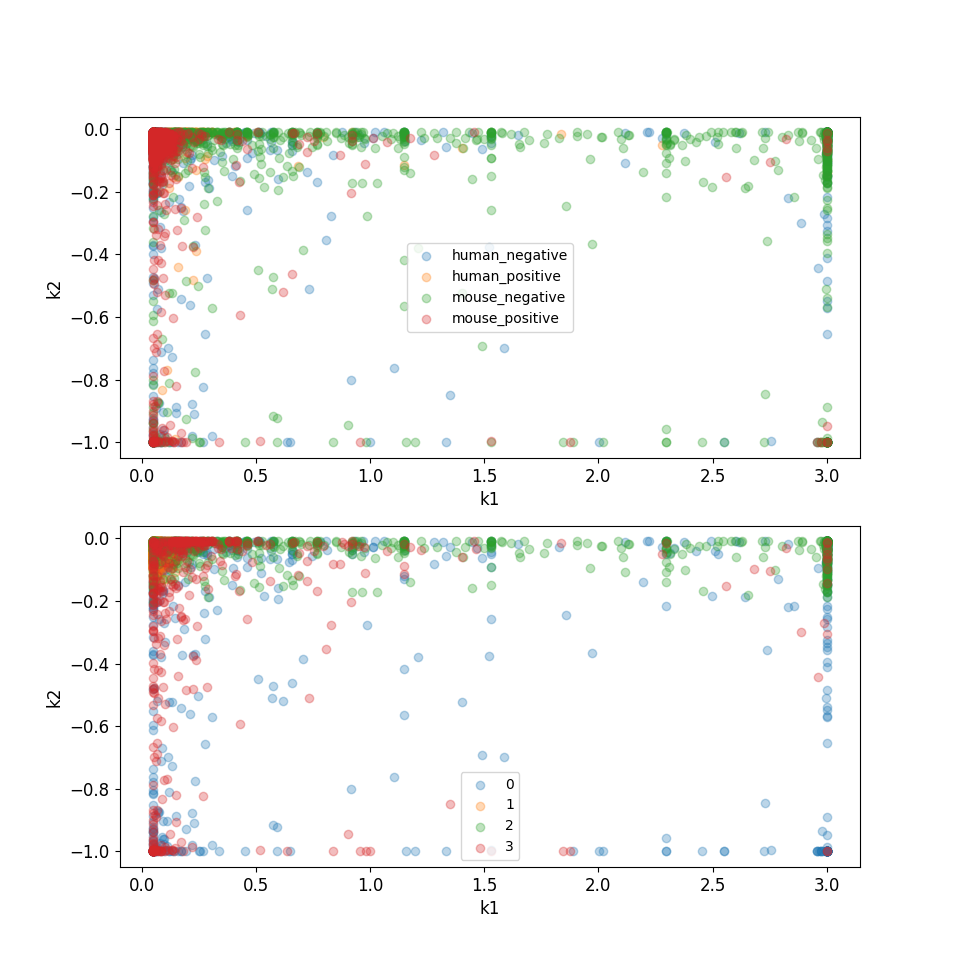
\includegraphics[width=\textwidth]{fig/seperate_k1_k2}
	\end{subfigure}
	\caption{Continuation of the visualization of the clustering results.}
\label{fig:vis_output_seperate3}
\end{figure}

\begin{figure}
	\begin{subfigure}{0.49\textwidth}
		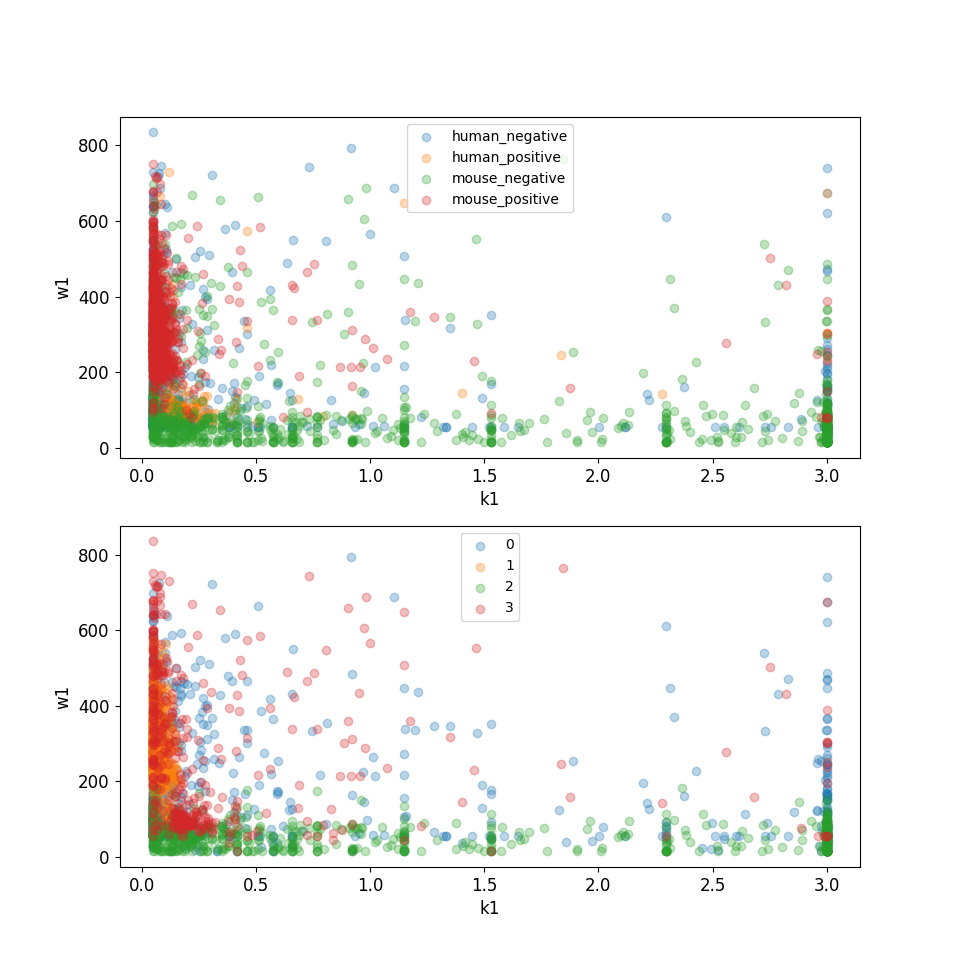
\includegraphics[width=\textwidth]{fig/seperate_k1_w1}
	\end{subfigure}
	\hfill
	\begin{subfigure}{0.49\textwidth}
		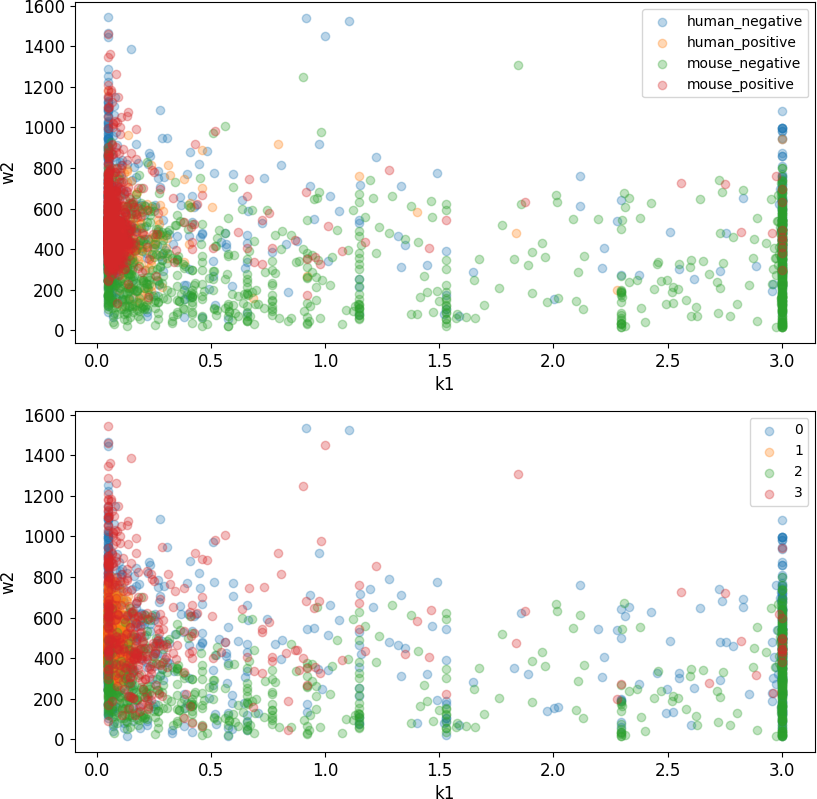
\includegraphics[width=\textwidth]{fig/seperate_k1_w2}
	\end{subfigure}
	\hfill
	\begin{subfigure}{0.49\textwidth}
		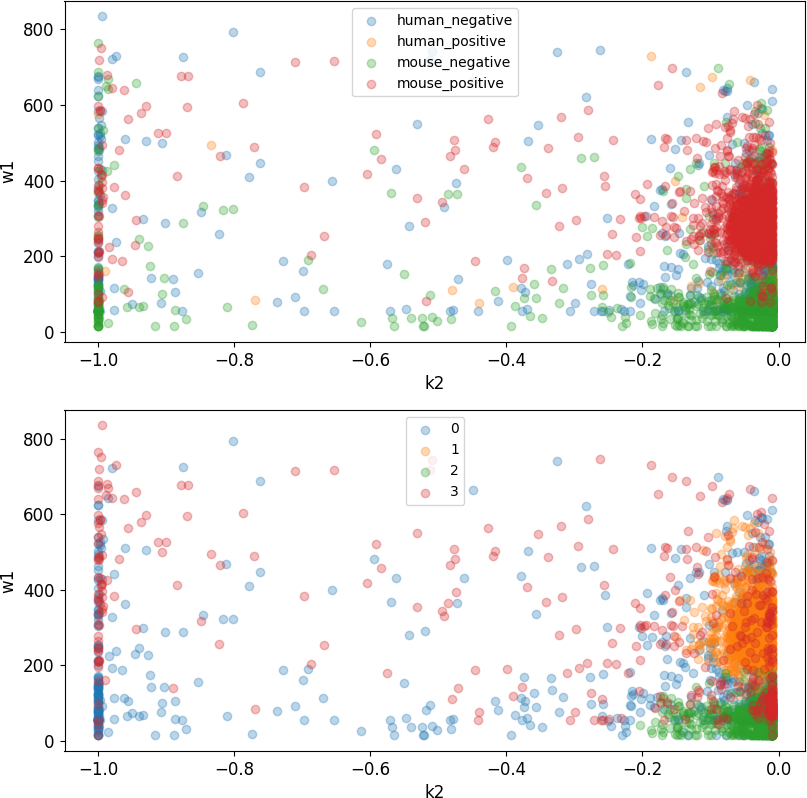
\includegraphics[width=\textwidth]{fig/seperate_k2_w1}
	\end{subfigure}
	\hfill
	\begin{subfigure}{0.49\textwidth}
		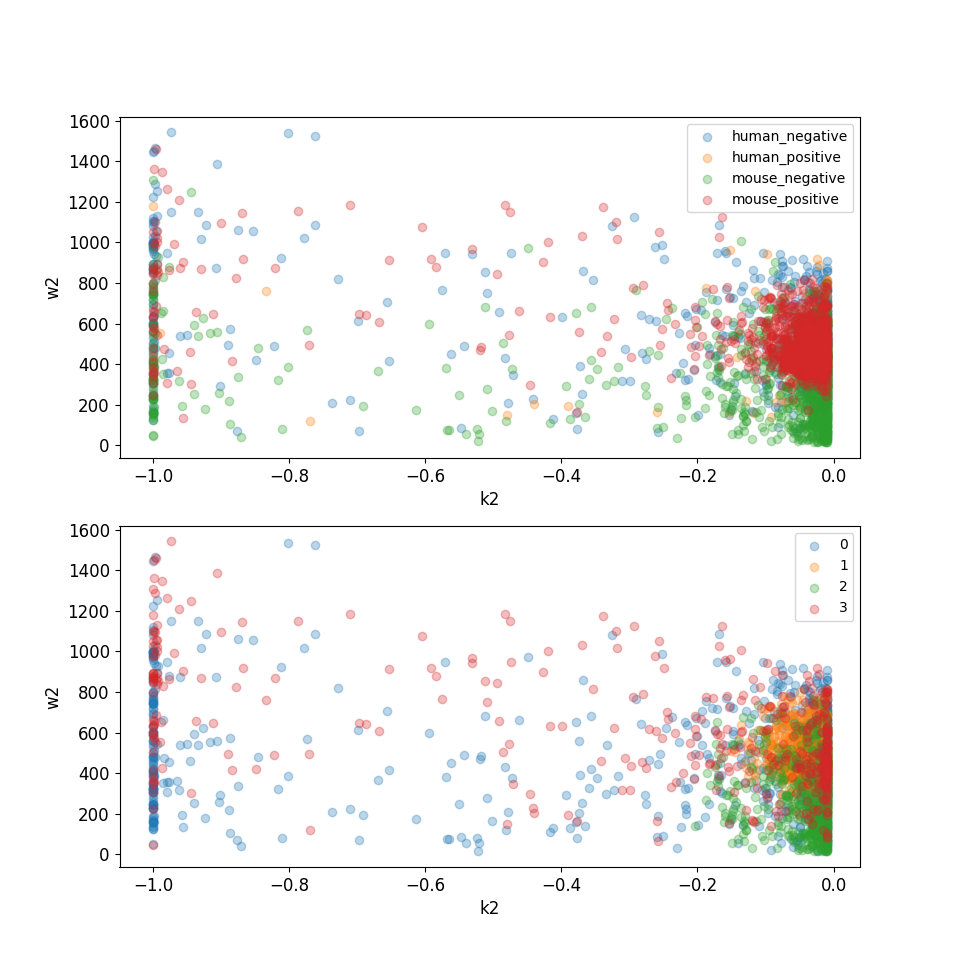
\includegraphics[width=\textwidth]{fig/seperate_k2_w2}
	\end{subfigure}
	\hfill
	\begin{subfigure}{0.49\textwidth}
		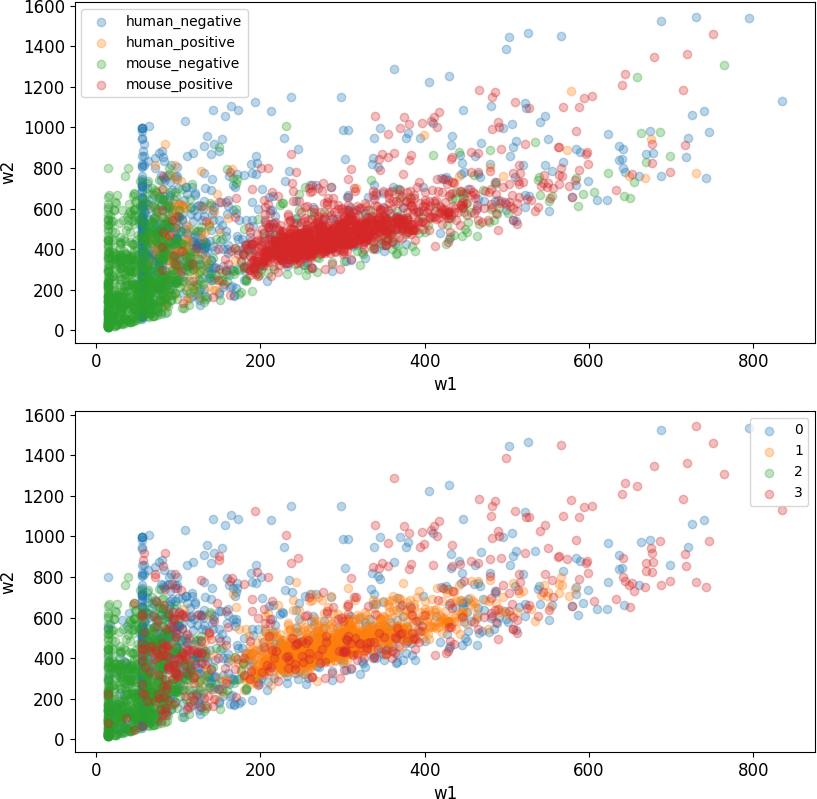
\includegraphics[width=\textwidth]{fig/seperate_w1_w2}
	\end{subfigure}
	
	\caption{Continuation of the visualization of the clustering results.}
	\label{fig:vis_output_seperate4}
\end{figure}

By comparing which data points are from which data set and where they were assigned by the Gaussian Mixture we can find an assignment between the two.

\newpage

The relevant information derived from the Gaussian Mixture clustering is the means and covariances of the four components. From this we can decide which cluster a new data point belongs to. A use case might be to find percentages of activated cells in an experiment. Distinguishing between mouse and human cells does not have a clear use case. When specifying \texttt{n\_components=2} we assume to have a cluster for activated and a second for unactivated cells.

Using the order of parameters $a, u, d, k_1, k_2, w_1$ and $w_2$ we get the mean and covariances for each of the data sets used in this work as 

\begin{align*}
	\text{human positive} && w = 0.148 && \mu = \left(\begin{matrix}
		2.429\\ 0.987\\ 1.703\\ 0.363\\	-0.275\\ 292.798\\ 587.26
	\end{matrix}\right) && \Sigma = diag\left(\begin{matrix}
		0.541\\ 0.245\\ 0.276\\ 0.395\\	0.131\\ 37561.179\\ 74216.954
	\end{matrix}\right),\\
	\text{human negative} && w = 0.278 && \mu = \left(\begin{matrix}
		0.735\\ 0.586\\ 0.612\\ 0.83\\ -0.267\\ 179.044\\ 491.68
	\end{matrix}\right) && \Sigma = diag\left(\begin{matrix}
		0.061\\ 0.029\\ 0.032\\ 1.347\\	0.144\\ 24314.336\\ 59213.616
	\end{matrix}\right),\\
	\text{mouse positive} && w = 0.346 && \mu = \left(\begin{matrix}
		3.111\\ 0.818\\ 1.676\\ 0.067\\ -0.038\\ 287.576\\ 480.405
	\end{matrix}\right) && \Sigma = diag\left(\begin{matrix}
		0.478\\ 0.016\\ 0.128\\ 0.0005\\ 0.0006\\ 7147.489\\ 10182.191
	\end{matrix}\right),\\
	\text{mouse negative} && w = 0.228 && \mu = \left(\begin{matrix}
		0.842\\ 0.762\\ 0.78\\ 1.335\\ -0.037\\ 56.052\\  285.085
	\end{matrix}\right) && \Sigma = diag\left(\begin{matrix}
	0.004\\ 0.002\\ 0.001\\ 1.513\\	0.002\\ 1149.598\\ 29471.53
	\end{matrix}\right).	
\end{align*}

When comparing these results to those of the average and standard deviation analysis done in table~\ref{tab:statistics_parameters} we can see similarities. However in comparison, to the approach focusing on outlier detection in section~\ref{sec:analysis_of_approximation} we now have an approach that is not only not dependent on parameters specified by a user, but can also be applied to a greater set of problems. A proposed way of answering the research questions from chapter~\ref{chapter:introduction} using these methods is described in chapter~\ref{chapter:results}.